\documentclass[11pt]{article}
\usepackage[margin=1in]{geometry}
\usepackage{amsmath,amssymb}
\usepackage{booktabs}
\usepackage{graphicx}
\usepackage{enumitem}

\title{CS555 HW1 -- Question 1: Observations}
\author{}
\date{}

\begin{document}
\maketitle

%----------------------------------------------------------------------
\section*{1a. Crank--Nicolson with $u^0 = \sin(\pi x)$}
%----------------------------------------------------------------------

\begin{table}[h!]
\centering
\caption{Euler Backward (EB) --- $u^0 = \sin(\pi x)$}
\begin{tabular}{rr cc}
\toprule
$N$ & nstep & $L_2$ error & ratio \\
\midrule
1500 &   25 & 7.69e-02 & --- \\
1500 &   50 & 3.87e-02 & 1.99 \\
1500 &  100 & 1.94e-02 & 1.99 \\
1500 &  200 & 9.72e-03 & 2.00 \\
1500 &  400 & 4.87e-03 & 2.00 \\
1500 &  800 & 2.43e-03 & 2.00 \\
1500 & 1600 & 1.22e-03 & 2.00 \\
\bottomrule
\end{tabular}
\end{table}

\begin{table}[h!]
\centering
\caption{Crank--Nicolson (CN) --- $u^0 = \sin(\pi x)$}
\begin{tabular}{rr cc}
\toprule
$N$ & nstep & $L_2$ error & ratio \\
\midrule
1500 &   25 & 1.03e-03 & --- \\
1500 &   50 & 2.56e-04 & 4.00 \\
1500 &  100 & 6.40e-05 & 4.00 \\
1500 &  200 & 1.59e-05 & 4.00 \\
1500 &  400 & 3.93e-06 & 4.06 \\
1500 &  800 & 9.34e-07 & 4.20 \\
1500 & 1600 & 2.42e-07 & 3.86 \\
\bottomrule
\end{tabular}
\end{table}

\begin{figure}[h!]
\centering
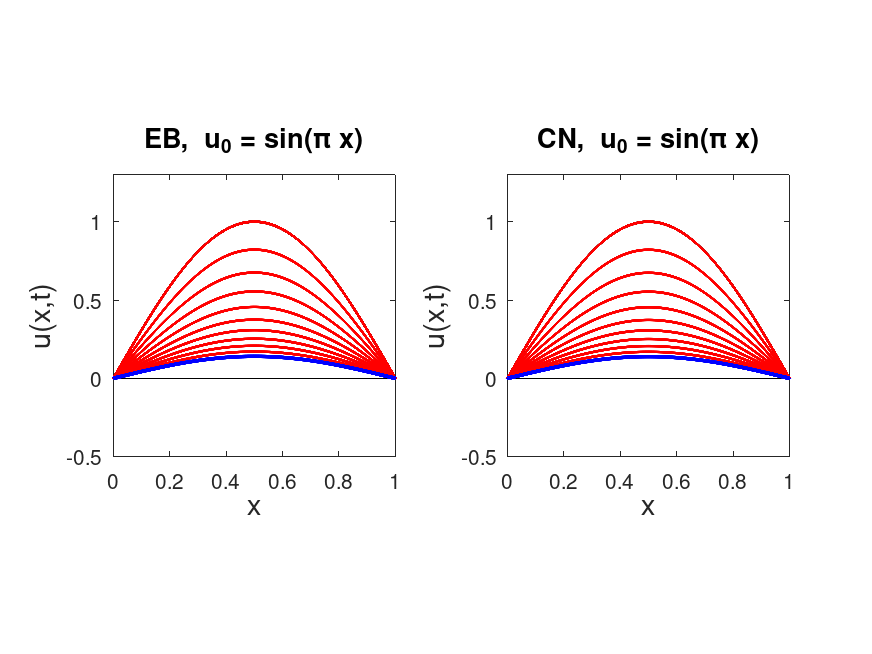
\includegraphics[width=0.95\textwidth]{plot_1a.png}
\caption{EB (left) vs.\ CN (right) with $u^0 = \sin(\pi x)$.
         Both methods produce smooth, oscillation-free solutions for this smooth IC.}
\end{figure}

\noindent\textbf{Observations:}
\begin{itemize}[nosep]
  \item \textbf{EB} shows error ratios converging to \textbf{2} as $\Delta t$ is halved,
        confirming \textbf{1st-order} accuracy in time (error $\propto \Delta t$).
  \item \textbf{CN} shows error ratios converging to \textbf{4} as $\Delta t$ is halved,
        confirming \textbf{2nd-order} accuracy in time (error $\propto \Delta t^2$).
        Halving $\Delta t$ reduces the error by a factor of $4 = 2^2$.
  \item CN is significantly more accurate than EB at the same $\Delta t$.
        For example, at nstep $= 100$, the CN error is roughly 300$\times$ smaller than the EB error.
\end{itemize}

\newpage
%----------------------------------------------------------------------
\section*{1b. Square wave IC: $u^0 = \pi/4$}
%----------------------------------------------------------------------

\begin{table}[h!]
\centering
\caption{Euler Backward (EB) --- $u^0 = \pi/4$}
\begin{tabular}{rr cc}
\toprule
$N$ & nstep & $L_2$ error & ratio \\
\midrule
1500 &   25 & 7.69e-02 & --- \\
1500 &   50 & 3.87e-02 & 1.99 \\
1500 &  100 & 1.94e-02 & 1.99 \\
1500 &  200 & 9.72e-03 & 2.00 \\
1500 &  400 & 4.87e-03 & 2.00 \\
1500 &  800 & 2.43e-03 & 2.00 \\
1500 & 1600 & 1.22e-03 & 2.00 \\
\bottomrule
\end{tabular}
\end{table}

\begin{table}[h!]
\centering
\caption{Crank--Nicolson (CN) --- $u^0 = \pi/4$}
\begin{tabular}{rr cc}
\toprule
$N$ & nstep & $L_2$ error & ratio \\
\midrule
1500 &   25 & 2.49e+00 & --- \\
1500 &   50 & 2.09e+00 & 1.19 \\
1500 &  100 & 1.75e+00 & 1.19 \\
1500 &  200 & 1.47e+00 & 1.19 \\
1500 &  400 & 1.23e+00 & 1.20 \\
1500 &  800 & 1.02e+00 & 1.20 \\
1500 & 1600 & 8.49e-01 & 1.20 \\
\bottomrule
\end{tabular}
\end{table}

\begin{figure}[h!]
\centering
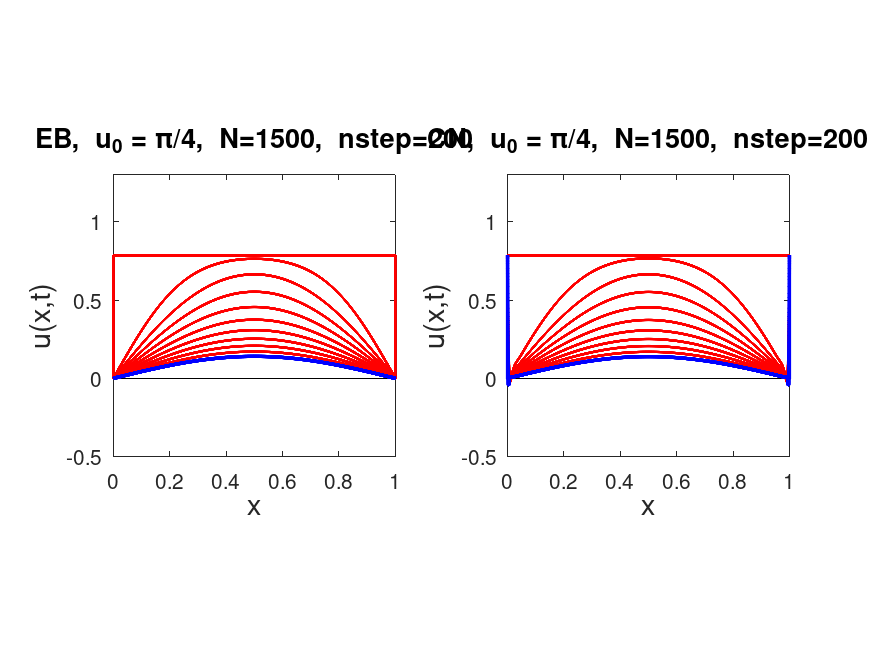
\includegraphics[width=0.95\textwidth]{plot_1b.png}
\caption{EB (left) vs.\ CN (right) with $u^0 = \pi/4$.
         CN exhibits persistent oscillations near the boundaries.}
\end{figure}

\noindent\textbf{Observations:}
\begin{itemize}[nosep]
  \item \textbf{EB} still converges with ratio $\approx 2$ (1st-order in time)
        even with the discontinuous IC.
        EB is \textbf{L-stable}: its growth factor $G = 1/(1+\lambda\Delta t) \to 0$
        as $\lambda\Delta t \to -\infty$, so it strongly damps all high-frequency
        Fourier modes excited by the boundary discontinuity.
  \item \textbf{CN fails to converge} properly.
        The errors are $O(1)$ and the ratio is $\approx 1.2$ instead of 4.
        CN is \textbf{A-stable but not L-stable}: its growth factor
        $G = (1 - \lambda\Delta t/2)/(1 + \lambda\Delta t/2) \to -1$
        as $\lambda\Delta t \to -\infty$.
        The high-frequency modes excited by the boundary discontinuity oscillate
        with amplitude $\approx 1$ and are never damped, producing persistent
        oscillations visible in the plot near $x=0$ and $x=1$.
  \item \textbf{Key lesson:} CN's 2nd-order accuracy advantage only applies to
        \textbf{smooth} initial conditions. For non-smooth data (like this square wave),
        EB's L-stability makes it more robust.
\end{itemize}

\newpage
%----------------------------------------------------------------------
\section*{1c. BDF2 (both ICs)}
%----------------------------------------------------------------------

\begin{table}[h!]
\centering
\caption{BDF2 --- $u^0 = \sin(\pi x)$}
\begin{tabular}{rr cc}
\toprule
$N$ & nstep & $L_2$ error & ratio \\
\midrule
1500 &   25 & 6.00e-04 & --- \\
1500 &   50 & 1.45e-04 & 4.13 \\
1500 &  100 & 3.61e-05 & 4.03 \\
1500 &  200 & 9.06e-06 & 3.98 \\
1500 &  400 & 2.33e-06 & 3.88 \\
1500 &  800 & 6.68e-07 & 3.49 \\
1500 & 1600 & 2.85e-07 & 2.34 \\
\bottomrule
\end{tabular}
\end{table}

\begin{table}[h!]
\centering
\caption{BDF2 --- $u^0 = \pi/4$}
\begin{tabular}{rr cc}
\toprule
$N$ & nstep & $L_2$ error & ratio \\
\midrule
1500 &   25 & 6.00e-04 & --- \\
1500 &   50 & 1.45e-04 & 4.13 \\
1500 &  100 & 3.60e-05 & 4.03 \\
1500 &  200 & 9.00e-06 & 4.00 \\
1500 &  400 & 2.27e-06 & 3.96 \\
1500 &  800 & 6.11e-07 & 3.72 \\
1500 & 1600 & 2.41e-07 & 2.53 \\
\bottomrule
\end{tabular}
\end{table}

\begin{figure}[h!]
\centering
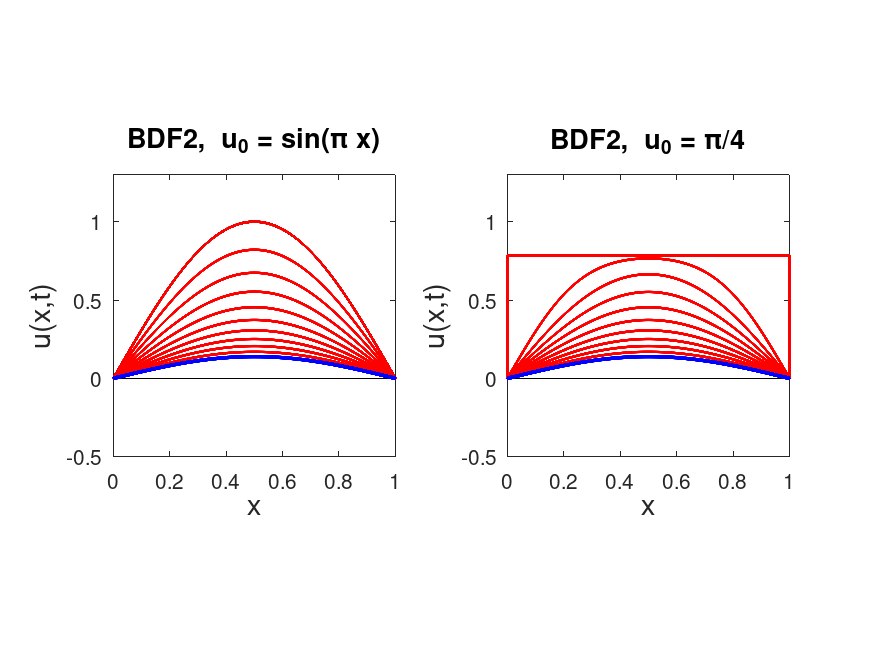
\includegraphics[width=0.95\textwidth]{plot_1c.png}
\caption{BDF2 with $u^0 = \sin(\pi x)$ (left) and $u^0 = \pi/4$ (right).
         No oscillations in either case.}
\end{figure}

\noindent\textbf{Observations:}
\begin{itemize}[nosep]
  \item \textbf{2nd-order convergence:} BDF2 shows error ratios approaching
        \textbf{4} as $\Delta t$ is halved for both ICs, confirming 2nd-order
        temporal accuracy---same order as CN.
  \item \textbf{L-stability advantage:} Unlike CN, BDF2 handles the discontinuous
        IC ($u^0 = \pi/4$) \textbf{without oscillations}. BDF2 is L-stable:
        $G \to 0$ as $\lambda\Delta t \to -\infty$, strongly damping high-frequency
        modes just like EB.
  \item \textbf{Both ICs give nearly identical errors:} Since BDF2 (like EB) damps
        the high-frequency modes that distinguish the two ICs, by $t=1$ both solutions
        are dominated by the $k=1$ Fourier mode and the errors are essentially the same.
  \item \textbf{Ratio degradation at fine $\Delta t$:} The ratio drops below 4 at the
        finest $\Delta t$ (nstep $= 800, 1600$). This is because the temporal error
        becomes comparable to the spatial discretization error at $N=1500$, so further
        $\Delta t$ refinement no longer gives pure temporal convergence.
  \item \textbf{BDF2 = best of both worlds:} It combines CN's 2nd-order accuracy
        with EB's L-stability, making it robust for non-smooth data while maintaining
        high-order convergence for smooth data.
\end{itemize}

\newpage
%----------------------------------------------------------------------
\section*{Extra Credit: Next leading-order term in the square wave}
%----------------------------------------------------------------------

The square wave $u^0 = \pi/4$ has the Fourier sine series
\[
  u^0 = \sum_{\substack{k=1,3,5,\ldots}} \frac{1}{k}\,\sin(k\pi x),
\]
so the exact solution is
\[
  u(x,t) = \sum_{\substack{k=1,3,5,\ldots}} \frac{1}{k}\,
            e^{-\nu(k\pi)^2 t}\,\sin(k\pi x).
\]

At $t=1$ with $\nu = 0.2$, the magnitudes of the leading Fourier coefficients are:

\begin{table}[h!]
\centering
\begin{tabular}{rc}
\toprule
$k$ & $\displaystyle\frac{1}{k}\,e^{-\nu(k\pi)^2}$ \\
\midrule
1 & $1.39 \times 10^{-1}$ \\
\textbf{3} & $\mathbf{6.42 \times 10^{-9}}$ \\
5 & $7.40 \times 10^{-23}$ \\
7 & $1.41 \times 10^{-43}$ \\
\bottomrule
\end{tabular}
\end{table}

\noindent
The next leading-order term ($k=3$) has magnitude
$\approx 6.4 \times 10^{-9}$, which is a factor of
$\approx 4.6 \times 10^{-8}$ smaller than the dominant $k=1$ mode.
The $k=3$ mode decays as $e^{-9\nu\pi^2}$ versus $e^{-\nu\pi^2}$ for $k=1$;
the $9\times$ larger exponent causes exponential suppression.

\medskip\noindent\textbf{Comparison to FD errors:}
\begin{itemize}[nosep]
  \item EB errors ($\sim 10^{-3}$): $\sim 10^5$ times \textbf{larger} than the $k=3$ term.
  \item BDF2 errors ($\sim 10^{-7}$): $\sim 10^2$ times \textbf{larger} than the $k=3$ term.
  \item CN errors ($\sim 10^{0}$): completely dominated by oscillations, irrelevant.
\end{itemize}

\medskip\noindent\textbf{Conclusion:}
The $k=3$ Fourier truncation error ($6.4 \times 10^{-9}$) is negligible compared to
all FD temporal errors in the preceding questions. This confirms that the assumption
$u(x,1) \approx e^{-\nu\pi^2}\sin(\pi x)$ (the $k=1$ eigenmode alone) is excellent.
The diffusion operator exponentially annihilates higher modes, and the time-stepping
error dominates in every case tested.

\end{document}
